\subsection{Random state and measurement preparation}
At the backbone of all classical protocols described in Section \ref{section:protocols}, it lies the need to generate random uniform distributions of either qubit states, Bloch vectors or shared randomness in $\mathbb{R^3}$. In Figure \ref{fig:results_random_states}, we can see that applying random unitary transformations to zero qubit states leads to uniformly distributed random qubit pure states, which can later be transformed into random Bloch vectors or normalized random vectors in $\mathbb{R^3}$ as needed. These random states are also the seed to compute random POVMs with rank-1 projectors, as described in Section \ref{section:povm_generation}. Hence, once proven we have means to generate random states and rank-1 POVMs, we can address the measurement process. 
\begin{figure}[h]
\centering
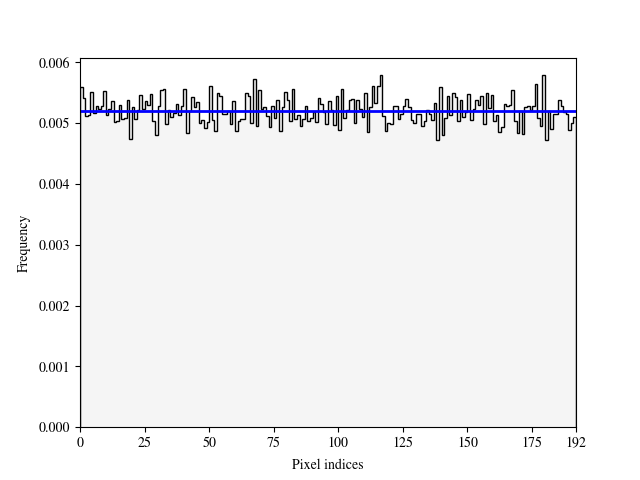
\includegraphics[width=0.9\textwidth]{images/random_bloch_healpix.png}
\caption{In this histogram we see how the frequency distribution of $N=10^4$ random qubit states generated with \cite{software2023} follows a random uniform distribution of state vectors along the Bloch sphere (blue solid line). The frequencies are binned by HEALPix indices corresponding to an equal-area iso-latitude partition of the Bloch sphere with resolution $\mathit{NSIDE}=4$.}
\label{fig:results_random_states}
\end{figure}

\subsection{Prepare-and-measure simulation outcomes}
The outcome probabilities for a given random POVM measure can be obtained analytically using the Born's rule, but we have gone a step further and used simulators and noisy intermediate-scale quantum computers (see Table \ref{table:quantum_resources}) to calculate such probabilities and compare them to the theoretical ones as described in Section \ref{section:quantum_circuit}. 
\newline
\begin{table}[h!]
\centering
{\renewcommand{\arraystretch}{1.2}%
\begin{tabular}{c c c c c} 
 \toprule
 Name & Qubits & Quantum Volume & CNOT Error & Readout Error \\ \hline
 Nairobi    & $\scriptstyle7$ 
            & $\scriptstyle32$ 
            & $\scriptstyle0.01357$ 
            & $\scriptstyle0.0227$ \\ \hline
 Perth      & $\scriptstyle7$ 
            & $\scriptstyle32$ 
            & $\scriptstyle0.01733$ 
            & $\scriptstyle0.0188$ \\ \hline
 Oslo       & $\scriptstyle7$ 
            & $\scriptstyle32$ 
            & $\scriptstyle0.01$ 
            & $\scriptstyle0.01667$ \\ \hline
 Jakarta    & $\scriptstyle7$ 
            & $\scriptstyle16$ 
            & $\scriptstyle0.00773$ 
            & $\scriptstyle0.0258$ \\ \hline
 Lagos      & $\scriptstyle7$ 
            & $\scriptstyle32$ 
            & $\scriptstyle0.007243$ 
            & $\scriptstyle0.0145$ \\ 
 \bottomrule
\end{tabular}}
\caption{Properties of Noisy Intermediate-Scale Quantum computers available at \href{https://quantum-computing.ibm.com}{IBM Quantum} to compute the prepare-and-measure outcome probabilities.}
\label{table:quantum_resources}
\end{table}

The quantum circuit resulting from applying Neumark's extension to a particular state and POVM measure is shown in Figure \ref{fig:quantum_circuit_example}. A summary of the achievable probability performances for such circuit using different quantum resources can be found in Table \ref{table:quantum_results}. Noisy quantum computers currently available to the public are limited to running circuits with a maximum of twenty thousand shots, so this results in less accuracy than desired. On the other hand, the Qiskit Aer simulator can perform noise-free simulations with a full range of shots, hence leading to better performances, as we will see later in the classical simulation results discussion. A full and comprehensive benchmark of IBM's free-access simulators and quantum computers for this prepare-and-measure scenario can be found in Appendix \ref{section:benchmark}.

\begin{figure}[!ht]
\centering
\begin{quantikz}
      \lstick{$\ket{\Psi}$}  & \gate[2][2cm]{U} & \meter{} \\
      \lstick{$\ket{0}$}  && \meter{} 
\end{quantikz}
\caption{Quantum circuit implementing a POVM measure of four elements. The unitary gate $U$ resulting from Neumark's is applied to the prepared state together with a single ancilla qubit such that the classical measurement leads to four possible outcomes: $\{00, 01, 10, 11\}$.}
\label{fig:quantum_circuit_example}
\end{figure}

A set of simulations have also been conducted for the prepare-and-measure classical protocol using a random assortment of states and measurements, in addition to a collection of well-known measures like the Cross-POVM (\ref{eq:cross-povm}), the Trine-POVM (\ref{eq:trine-povm}) and a four-element SIC-POVM sample (\ref{eq:sic-povm}). 

\begin{landscape}
\topskip0pt
\vspace*{\fill}
\begin{tabular}{c|cccc|cccc|cccc|cccc}
\toprule
\textbf{Shots}  & \multicolumn{4}{c|}{$\scriptstyle10^2$} 
                & \multicolumn{4}{c|}{$\scriptstyle10^3$} 
                & \multicolumn{4}{c|}{$\scriptstyle10^4$} 
                & \multicolumn{4}{c}{$\scriptstyle2\cdot 10^4$}\\
\midrule
\textbf{Measure}    & $\scriptstyle00$ & $\scriptstyle01$ & $\scriptstyle10$ & $\scriptstyle11$
                    & $\scriptstyle00$ & $\scriptstyle01$ & $\scriptstyle10$ & $\scriptstyle11$
                    & $\scriptstyle00$ & $\scriptstyle01$ & $\scriptstyle10$ & $\scriptstyle11$
                    & $\scriptstyle00$ & $\scriptstyle01$ & $\scriptstyle10$ & $\scriptstyle11$\\
\midrule
Aer Simulator   & $\scriptstyle0.370$ & $\scriptstyle0.150$ & $\scriptstyle0.070$ & $\scriptstyle0.410$ 
                & $\scriptstyle0.362$ & $\scriptstyle0.117$ & $\scriptstyle0.067$ & $\scriptstyle0.454$ 
                & $\scriptstyle0.377$ & $\scriptstyle0.122$ & $\scriptstyle0.062$ & $\scriptstyle0.438$ 
                & $\scriptstyle0.378$ & $\scriptstyle0.120$ & $\scriptstyle0.058$ & $\scriptstyle0.443$\\                
Nairobi         & $\scriptstyle0.400$ & $\scriptstyle0.140$ & $\scriptstyle0.030$ & $\scriptstyle0.430$ 
                & $\scriptstyle0.335$ & $\scriptstyle0.162$ & $\scriptstyle0.112$ & $\scriptstyle0.391$ 
                & $\scriptstyle0.378$ & $\scriptstyle0.172$ & $\scriptstyle0.090$ & $\scriptstyle0.359$
                & $\scriptstyle0.345$ & $\scriptstyle0.115$ & $\scriptstyle0.097$ & $\scriptstyle0.443$\\               
Perth           & $\scriptstyle0.350$ & $\scriptstyle0.260$ & $\scriptstyle0.100$ & $\scriptstyle0.290$ 
                & $\scriptstyle0.337$ & $\scriptstyle0.185$ & $\scriptstyle0.121$ & $\scriptstyle0.357$ 
                & $\scriptstyle0.370$ & $\scriptstyle0.187$ & $\scriptstyle0.118$ & $\scriptstyle0.325$
                & $\scriptstyle0.328$ & $\scriptstyle0.152$ & $\scriptstyle0.113$ & $\scriptstyle0.408$\\
Oslo            & $\scriptstyle0.400$ & $\scriptstyle0.080$ & $\scriptstyle0.040$ & $\scriptstyle0.480$ 
                & $\scriptstyle0.379$ & $\scriptstyle0.100$ & $\scriptstyle0.052$ & $\scriptstyle0.469$ 
                & $\scriptstyle0.358$ & $\scriptstyle0.108$ & $\scriptstyle0.070$ & $\scriptstyle0.463$
                & $\scriptstyle0.378$ & $\scriptstyle0.114$ & $\scriptstyle0.064$ & $\scriptstyle0.444$\\
Jakarta         & $\scriptstyle0.350$ & $\scriptstyle0.160$ & $\scriptstyle0.110$ & $\scriptstyle0.380$ 
                & $\scriptstyle0.378$ & $\scriptstyle0.160$ & $\scriptstyle0.076$ & $\scriptstyle0.386$ 
                & $\scriptstyle0.383$ & $\scriptstyle0.143$ & $\scriptstyle0.088$ & $\scriptstyle0.386$
                & $\scriptstyle0.366$ & $\scriptstyle0.149$ & $\scriptstyle0.099$ & $\scriptstyle0.387$\\   
Lagos           & $\scriptstyle0.380$ & $\scriptstyle0.100$ & $\scriptstyle0.060$ & $\scriptstyle0.460$ 
                & $\scriptstyle0.366$ & $\scriptstyle0.113$ & $\scriptstyle0.060$ & $\scriptstyle0.461$ 
                & $\scriptstyle0.357$ & $\scriptstyle0.113$ & $\scriptstyle0.062$ & $\scriptstyle0.467$
                & $\scriptstyle0.366$ & $\scriptstyle0.130$ & $\scriptstyle0.070$ & $\scriptstyle0.434$\\
\midrule
\textbf{Born's rule}    & $\scriptstyle0.375$ & $\scriptstyle0.125$ & $\scriptstyle0.064$ & $\scriptstyle0.435$ 
                        & $\scriptstyle0.375$ & $\scriptstyle0.125$ & $\scriptstyle0.064$ & $\scriptstyle0.435$ 
                        & $\scriptstyle0.375$ & $\scriptstyle0.125$ & $\scriptstyle0.064$ & $\scriptstyle0.435$ 
                        & $\scriptstyle0.375$ & $\scriptstyle0.125$ & $\scriptstyle0.064$ & $\scriptstyle0.435$ \\
\bottomrule        
\end{tabular}
\captionof{table}{Example of probability distributions for circuit's classical measurement outcomes $\{00, 01, 10, 11\}$ obtained with different IBM Quantum systems and simulators. The prepare-and-measure scenario is that with state $\ket{\Psi}=\frac{3 + i \sqrt{3}}{4} \ket{0} - \frac{1}{2} \ket{1}$ and POVM measure $\mathbb{P}_4 = \{\frac{1}{2}\ket{0}\bra{0}, \frac{1}{2}\ket{1}\bra{1}, \frac{1}{2}\ket{+}\bra{+}, \frac{1}{2}\ket{-}\bra{-} \}$.}
\label{table:quantum_results}
\vspace*{\fill}
\end{landscape}

The results shown in Table \ref{table:classical_results_pm} clearly indicate that the correlations obtained by the classical prepare-and-measure simulations reproduce the quantum probabilities with extraordinary accuracy. The relative entropy distances among the theoretical probability distribution $P$, and the classical simulation probability distribution $Q$, on the sample space $\mathcal{X}$, have also been computed following the Kullback-Leibler divergence formula \cite{mackay2003}
\begin{equation}\label{eq:kullback}
D_{KL}(P||Q) = \sum_{x\in \mathcal{X}}{P(x)\ log\frac{P(x)}{Q(x)}}
\end{equation}
Figure \ref{fig:classical_results_kl} shows the Kullback-Leibler divergence among Born's rule and the classical simulation probabilities obtained for the set of prepare-and-measure scenarios in Table \ref{table:classical_results_pm}.
\newline
\begin{table}[h!]
\centering
{\renewcommand{\arraystretch}{1.5}%
\begin{tabular}{ccccc} 
 \toprule
 Scenario & \multicolumn{4}{c}{Probabilities}  \\ \hline
 {Cross-POVM$^1$}   & $\scriptstyle0.3749^{\textcolor[rgb]{0,0,1}{0.3750}}$ 
                    & $\scriptstyle0.1250^{\textcolor[rgb]{0,0,1}{0.1250}}$ 
                    & $\scriptstyle0.0625^{\textcolor[rgb]{0,0,1}{0.0625}}$ 
                    & $\scriptstyle0.4376^{\textcolor[rgb]{0,0,1}{0.4375}}$ \\ \hline
 {Trine-POVM$^2$}   & $\scriptstyle0.4998^{\textcolor[rgb]{0,0,1}{0.5000}}$ 
                    & $\scriptstyle0.0335^{\textcolor[rgb]{0,0,1}{0.0335}}$ 
                    & $\scriptstyle0.4667^{\textcolor[rgb]{0,0,1}{0.4665}}$ 
                    & -  \\ \hline
 {SIC-POVM$^3$}     & $\scriptstyle0.3751^{\textcolor[rgb]{0,0,1}{0.3750}}$ 
                    & $\scriptstyle0.0315^{\textcolor[rgb]{0,0,1}{0.0316}}$ 
                    & $\scriptstyle0.3851^{\textcolor[rgb]{0,0,1}{0.3851}}$ 
                    & $\scriptstyle0.2082^{\textcolor[rgb]{0,0,1}{0.2083}}$ \\ \hline
 {Random-PVM$^4$}   & $\scriptstyle0.9669^{\textcolor[rgb]{0,0,1}{0.9669}}$ 
                    & $\scriptstyle0.0331^{\textcolor[rgb]{0,0,1}{0.0331}}$ 
                    & - 
                    & - \\ \hline
 {Random-POVM$^5$}  & $\scriptstyle0.0097^{\textcolor[rgb]{0,0,1}{0.0097}}$ 
                    & $\scriptstyle0.0057^{\textcolor[rgb]{0,0,1}{0.0057}}$ 
                    & $\scriptstyle0.8825^{\textcolor[rgb]{0,0,1}{0.8825}}$ 
                    & $\scriptstyle0.1021^{\textcolor[rgb]{0,0,1}{0.1021}}$ \\ \hline
 {Random-POVM$^6$}  & $\scriptstyle0.2386^{\textcolor[rgb]{0,0,1}{0.2389}}$ 
                    & $\scriptstyle0.1242^{\textcolor[rgb]{0,0,1}{0.1242}}$ 
                    & $\scriptstyle0.6341^{\textcolor[rgb]{0,0,1}{0.6337}}$ 
                    & $\scriptstyle0.0031^{\textcolor[rgb]{0,0,1}{0.0031}}$\\
 \bottomrule
\end{tabular}}
\caption{Probability outcomes of several prepare-and-measure classical simulations after $10^7$ shots, and using a diverse set of measurements and prepared states $\ket{\Psi}$. For the purpose of comparison, theoretical probabilities calculated using Born's rule are presented in superscript blue color. \\$^{1,2,3}\:\ket{\Psi}=\frac{3 + i \sqrt{3}}{4} \ket{0} - \frac{1}{2} \ket{1}$\\
$^{4,5}\:\ket{\Psi}= - (0.606 + 0.642 i) \ket{0} - (0.336 + 0.327i) \ket{1}$\\
$^{6}\:\ket{\Psi}= (-0.461 + 0.195i) \ket{0} - (0.767 - 0.402i) \ket{1}$}
\label{table:classical_results_pm}
\end{table}

\begin{figure}[h!]
\centering
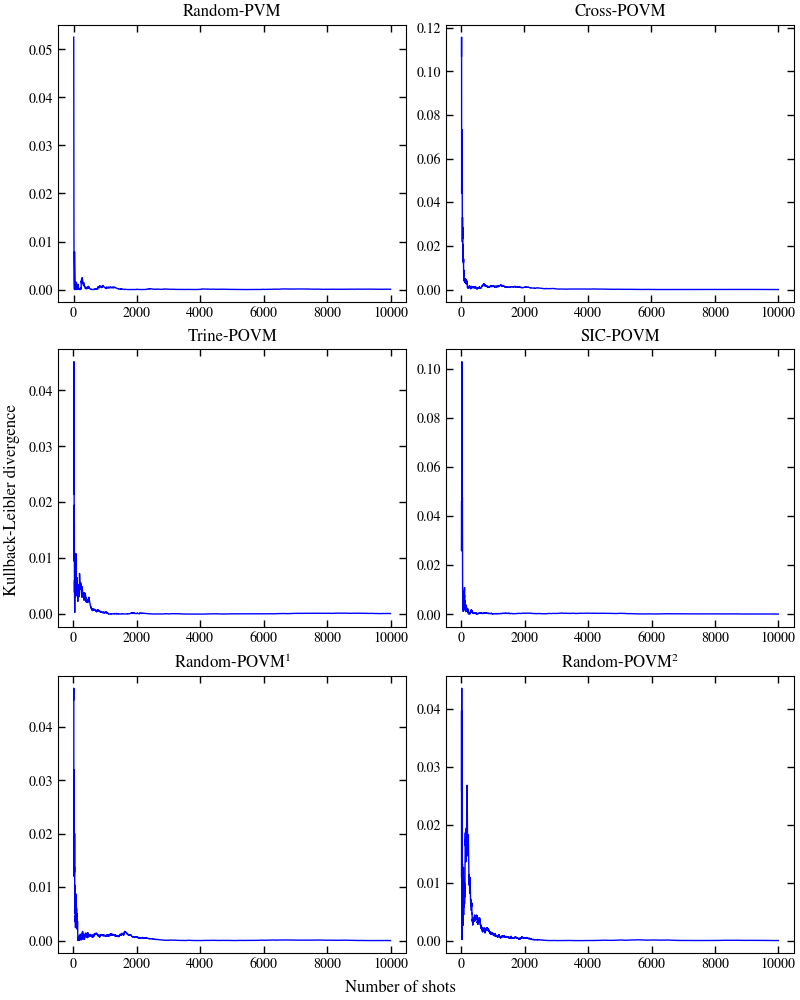
\includegraphics[width=\textwidth]{images/pm_povm_kl.png}
\caption{The Kullback-Leibler relative entropy among the theoretical probabilities and the simulation probability distributions for the prepare-and-measure scenarios specified in Table \ref{table:classical_results_pm}. A total of $10^4$ shots were used for the simulations, and it can be clearly seen that the results converge to zero statistical distance rather quickly.}
\label{fig:classical_results_kl}
\end{figure}

\subsection{Bell simulation outcomes}
Taking advantage of the analysis performed comparing theoretical and simulated probability distributions, we have extended the variational distance analysis to the prepare-and-measure scenario using IBM Quantum simulators. Figure \ref{fig:classical_quantum_results_kl} shows that existing quantum simulators converge to the expected theoretical values slightly slower than the classical simulations. The outcome probabilities after $10^7$ simulation runs are available in Table \ref{table:classical_quantum_results}.

\begin{figure}[h!]
\centering
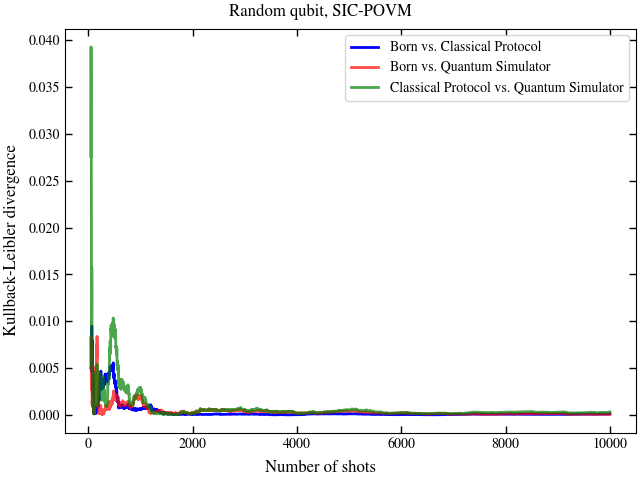
\includegraphics[width=0.7\textwidth]{images/pm_povm_kl_bcq.png}
\caption{The Kullback-Leibler relative entropy among the theoretical probabilities and the simulation probability distributions using the classical protocol and the IBM Quantum simulator. The prepared state selected is $\ket{\Psi}=3/4 + i \sqrt{3}/4 \ket{0} - 1/2 \ket{1}$, and the POVM measure the four-element Cross-POVM (\ref{eq:cross-povm}). A total of $10^4$ shots were used for the simulations, where it can be noticed some differences in the convergence, particularly during the first thousands of runs.}
\label{fig:classical_quantum_results_kl}
\end{figure}

\begin{table}[h!]
\centering
{\renewcommand{\arraystretch}{1.2}%
\begin{tabular}{c c c c c} 
 \toprule
 Method & \multicolumn{4}{c}{Probabilities}  \\ \hline
 Classical Simulation   & $\scriptstyle0.3749$ 
                        & $\scriptstyle0.1250$ 
                        & $\scriptstyle0.0625$ 
                        & $\scriptstyle0.4376$ \\ \hline 
 Quantum Simulation     & $\scriptstyle0.3751$ 
                        & $\scriptstyle0.1249$ 
                        & $\scriptstyle0.0625$ 
                        & $\scriptstyle0.4374$ \\ \hline
 Born's rule            & $\scriptstyle0.3750$ 
                        & $\scriptstyle0.1250$ 
                        & $\scriptstyle0.0625$ 
                        & $\scriptstyle0.4375$ \\ 
 \bottomrule
\end{tabular}}
\caption{Probability outcomes of prepare-and-measure classical and quantum simulations after $10^{7}$ shots. The prepared state selected is $\ket{\Psi}=3/4 + i \sqrt{3}/4 \ket{0} - 1/2 \ket{1}$, and the POVM measure the four-element Cross-POVM (\ref{eq:cross-povm}). The theoretical probabilities obtained applying Born’s rule are also
provided for ease of comparison.}
\label{table:classical_quantum_results}
\end{table}

Following the protocol described in Section \ref{section:protocol_bell}, and the corresponding methodology in Section \ref{section:methods_bell}, a complementary set of simulations have also been carried out for a Bell scenario with a singlet state and local projective measurements. Similarly to the prepare-and-measure scenario case, the results in Table \ref{table:classical_results_bell} show that the correlations obtained by the classical Bell simulations reproduce the quantum joint probabilities and expectation values with remarkable accuracy. In Table \ref{table:classical_results_bell} it is straightforward to see that, in the classical simulation performed, the CHSH inequality is violated in the chosen set of Alice and Bob observables, and it is therefore consistent with quantum theory predictions. 

The convergence of joint probabilities to theoretical values is illustrated more visually in Figure \ref{fig:classical_results_bell}, which demonstrates a rapid convergence as the number of shots increases. On the other hand, Figure \ref{fig:classical_theoretical_results_bell} exhibits the accuracy of this convergence to the theoretical values.

\begin{table}[h!]
\centering
{\renewcommand{\arraystretch}{1.5}%
\begin{tabular}{c | c | c | c | c | c} 
 \toprule
 \multirow{2}*{$(a_x, b_y)$} & \multicolumn{4}{c|}{$p_C(a_x, b_y|A_x,B_y)$} & \multirow{2}*{CHSH} \\ \cline{2-5}
 & $(A_0, B_0)$ & $(A_0, B_1)$ & $(A_1, B_0)$ & $(A_1, B_1)$ & \\ \hline
 $(+1, +1)$ & $\scriptstyle0.4268^{\textcolor[rgb]{0,0,1}{0.4267}}$ 
            & $\scriptstyle0.4269^{\textcolor[rgb]{0,0,1}{0.4267}}$ 
            & $\scriptstyle0.4267^{\textcolor[rgb]{0,0,1}{0.4267}}$
            & $\scriptstyle0.0734^{\textcolor[rgb]{0,0,1}{0.0732}}$ & -\\ \hline
$(+1, -1)$  & $\scriptstyle0.0731^{\textcolor[rgb]{0,0,1}{0.0732}}$ 
            & $\scriptstyle0.0732^{\textcolor[rgb]{0,0,1}{0.0732}}$  
            & $\scriptstyle0.0732^{\textcolor[rgb]{0,0,1}{0.0732}}$ 
            & $\scriptstyle0.4265^{\textcolor[rgb]{0,0,1}{0.4267}}$ & -\\ \hline
$(-1, +1)$  & $\scriptstyle0.0732^{\textcolor[rgb]{0,0,1}{0.0732}}$ 
            & $\scriptstyle0.0733^{\textcolor[rgb]{0,0,1}{0.0732}}$ 
            & $\scriptstyle0.0732^{\textcolor[rgb]{0,0,1}{0.0732}}$ 
            & $\scriptstyle0.4270^{\textcolor[rgb]{0,0,1}{0.4267}}$ & -\\ \hline
$(-1, -1)$  & $\scriptstyle0.4268^{\textcolor[rgb]{0,0,1}{0.4267}}$
            & $\scriptstyle0.4267^{\textcolor[rgb]{0,0,1}{0.4267}}$ 
            & $\scriptstyle0.4269^{\textcolor[rgb]{0,0,1}{0.4267}}$ 
            & $\scriptstyle0.0731^{\textcolor[rgb]{0,0,1}{0.0732}}$ & -\\ \hline
$\mathbb{E}[A_x, B_y]$  & $\scriptstyle{0.7072}$ 
                        & $\scriptstyle{0.7073}$ 
                        & $\scriptstyle{0.7072}$ 
                        & $\scriptstyle{-0.7070}$ 
                        & $\scriptstyle{2.8287}$\\
\bottomrule
\end{tabular}}
\caption{Probability outcomes of a classical Bell simulation after $10^{7}$ shots. The entanglement state is the Bell singlet state $\ket{\Psi^{-}}=(\ket{00} - \ket{11})/\sqrt{2}$, and the observables chosen are $A_0=Z,\:A_1=X,\:B_0=-(X +Z)/\sqrt{2},\:B_1=(X - Z)1/\sqrt{2}$. For the purpose of comparison, theoretical probabilities calculated using Born's rule are presented in superscript blue color.}
\label{table:classical_results_bell}
\end{table}

\begin{figure}[h!]
\centering
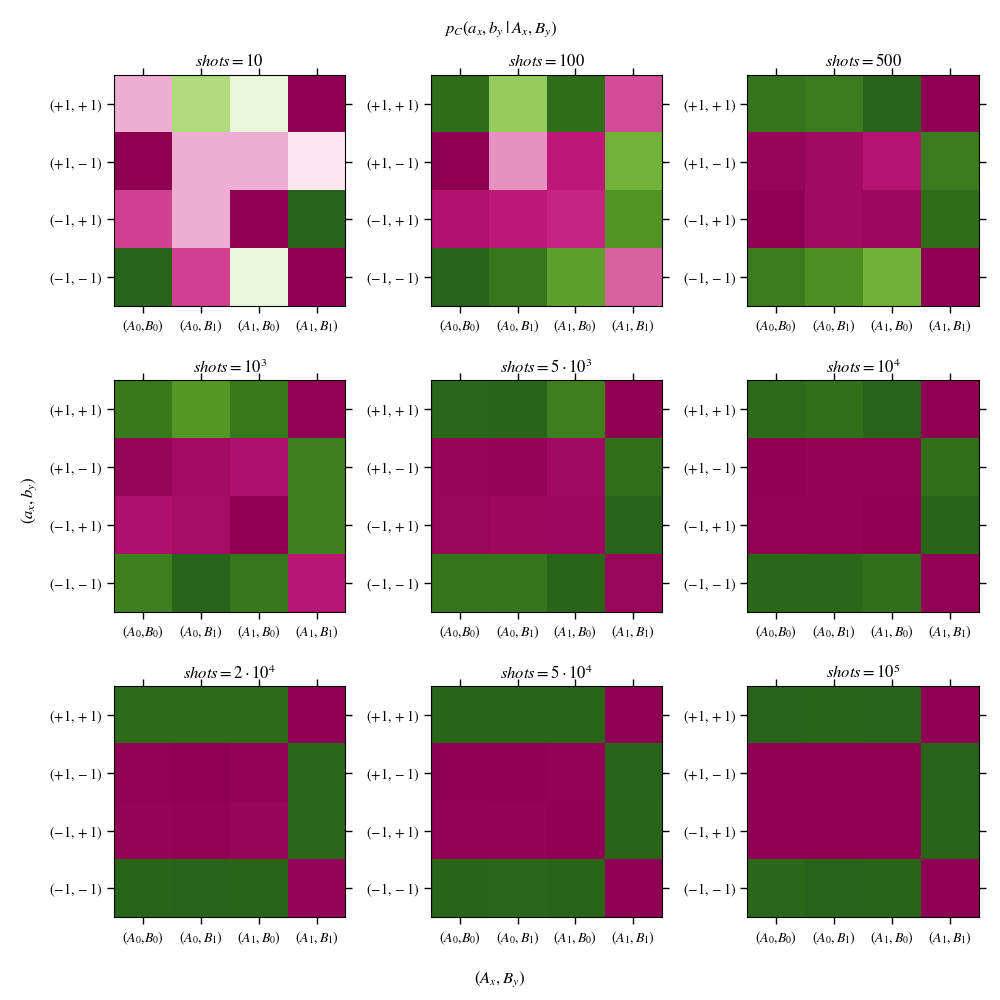
\includegraphics[width=\textwidth]{images/bell_heatmap_classical.png}
\caption{The joint probabilities for the Bell classical simulations are plotted in a heatmap for various numbers of shots, revealing that the outcomes begin to converge after a few thousand shots.}
\label{fig:classical_results_bell}
\end{figure}

\begin{figure}[h!]
\centering
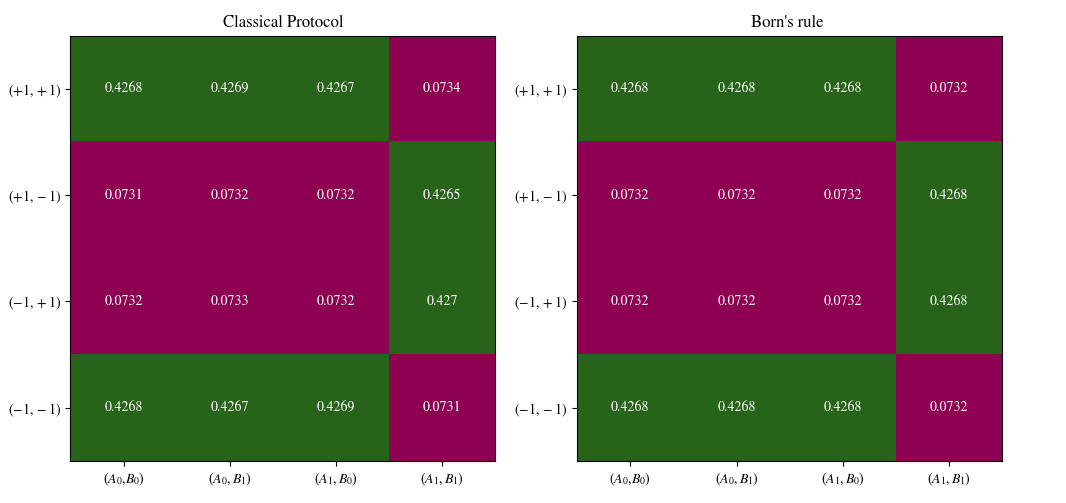
\includegraphics[width=\textwidth]{images/bell_heatmap_classical_theoretical.png}
\caption{The heatmap displays the joint probabilities obtained from a classical Bell simulation after $10^7$ shots, alongside the theoretical values computed via Born's rule, revealing a significant level of accuracy.}
\label{fig:classical_theoretical_results_bell}
\end{figure}
\clearpage